\documentclass[handout,nooutcomes]{ximera}
%% handout
%% space
%% newpage
%% numbers
%% nooutcomes


\newcommand{\RR}{\mathbb R}
\renewcommand{\d}{\,d}
\newcommand{\dd}[2][]{\frac{d #1}{d #2}}
\renewcommand{\l}{\ell}
\newcommand{\ddx}{\frac{d}{dx}}
\newcommand{\dfn}{\textbf}
\newcommand{\eval}[1]{\bigg[ #1 \bigg]}

\usepackage{multicol}

\renewenvironment{freeResponse}{
\ifhandout\setbox0\vbox\bgroup\else
\begin{trivlist}\item[\hskip \labelsep\bfseries Solution:\hspace{2ex}]
\fi}
{\ifhandout\egroup\else
\end{trivlist}
\fi} %% we can turn off input when making a master document

\title{Recitation \#8 - 3.2 Working with Derivatives}  

\begin{document}
\begin{abstract}		\end{abstract}
\maketitle

\section*{Warm up:} 
	
	\begin{enumerate}
	
	%part 1
	\item[(1)] If $f'(2)$ exists, then $\lim_{x \to 2} f(x)$
	
		\begin{enumerate}
		
		\item must exist, but more information is needed if we want to find it.
		
		\item is equal to $f(2)$.
		
		\item is equal to $f'(2)$.
		
		\item need not exist.
		
		\end{enumerate}
	
			\begin{freeResponse}
			The correct answer is (b).  If $f'(2)$ exists, then the function $f(x)$ is differentiable at $x=2$.  There is a theorem that says ``if $f(x)$ is differentiable at $x=a$, then $f(x)$ is continuous at $x=a$".  So $f(x)$ is continuous at $x=2$, and by definition, this means that $\lim_{x \to 2} f(x) = f(2)$.
			\end{freeResponse}
	
	%part 2
	\item[(2)]  Assuming that $\lim_{x \to 0} \frac{\sin x}{x} = 1$, we can conclude
	
		\begin{enumerate}
		
		\item $\frac{0}{0} = 1$.
		
		\item the tangent line to $y = \sin x$ at $(0,0)$ has slope $1$.
		
		\item you can cancel the $x$'s.
		
		\item for all $x$ near $0$, $\sin x = x$.
		
		\item for all $x$ near $0$, $\sin x \approx x$.
		
		\end{enumerate} 
	
			\begin{freeResponse}
			The answers are (b) and (e).  To see that (b) is true, if we write out the limit definition of the derivative of $f(x) = \sin x$ at $x=0$, we get that 
			$f'(0) = \lim_{h \to 0} \frac{\sin (h + 0) - \sin (0)}{h}
			= \lim_{h \to 0} \frac{\sin (h)}{h}$.  
			But this equals $1$ by the assumption, and so the tangent line to the graph of $y = \sin(x)$ at $(0,0)$ has slope $1$.  
			
			For (e), note that this is what it means for $y=x$ to be the tangent line to the graph of $y = \sin(x)$ at $x=0$.
			\end{freeResponse}
		
	\end{enumerate}
	
	
	
	
	
	

\section*{Group work:}

%problem 1
\begin{problem}
Look at the following work for finding the derivative of $f(x) = \frac{x}{x-5}$ at the point $x=3$ using the definition of the derivative.  Adapt the following work to find $f'(x)$.  
	\begin{image}
	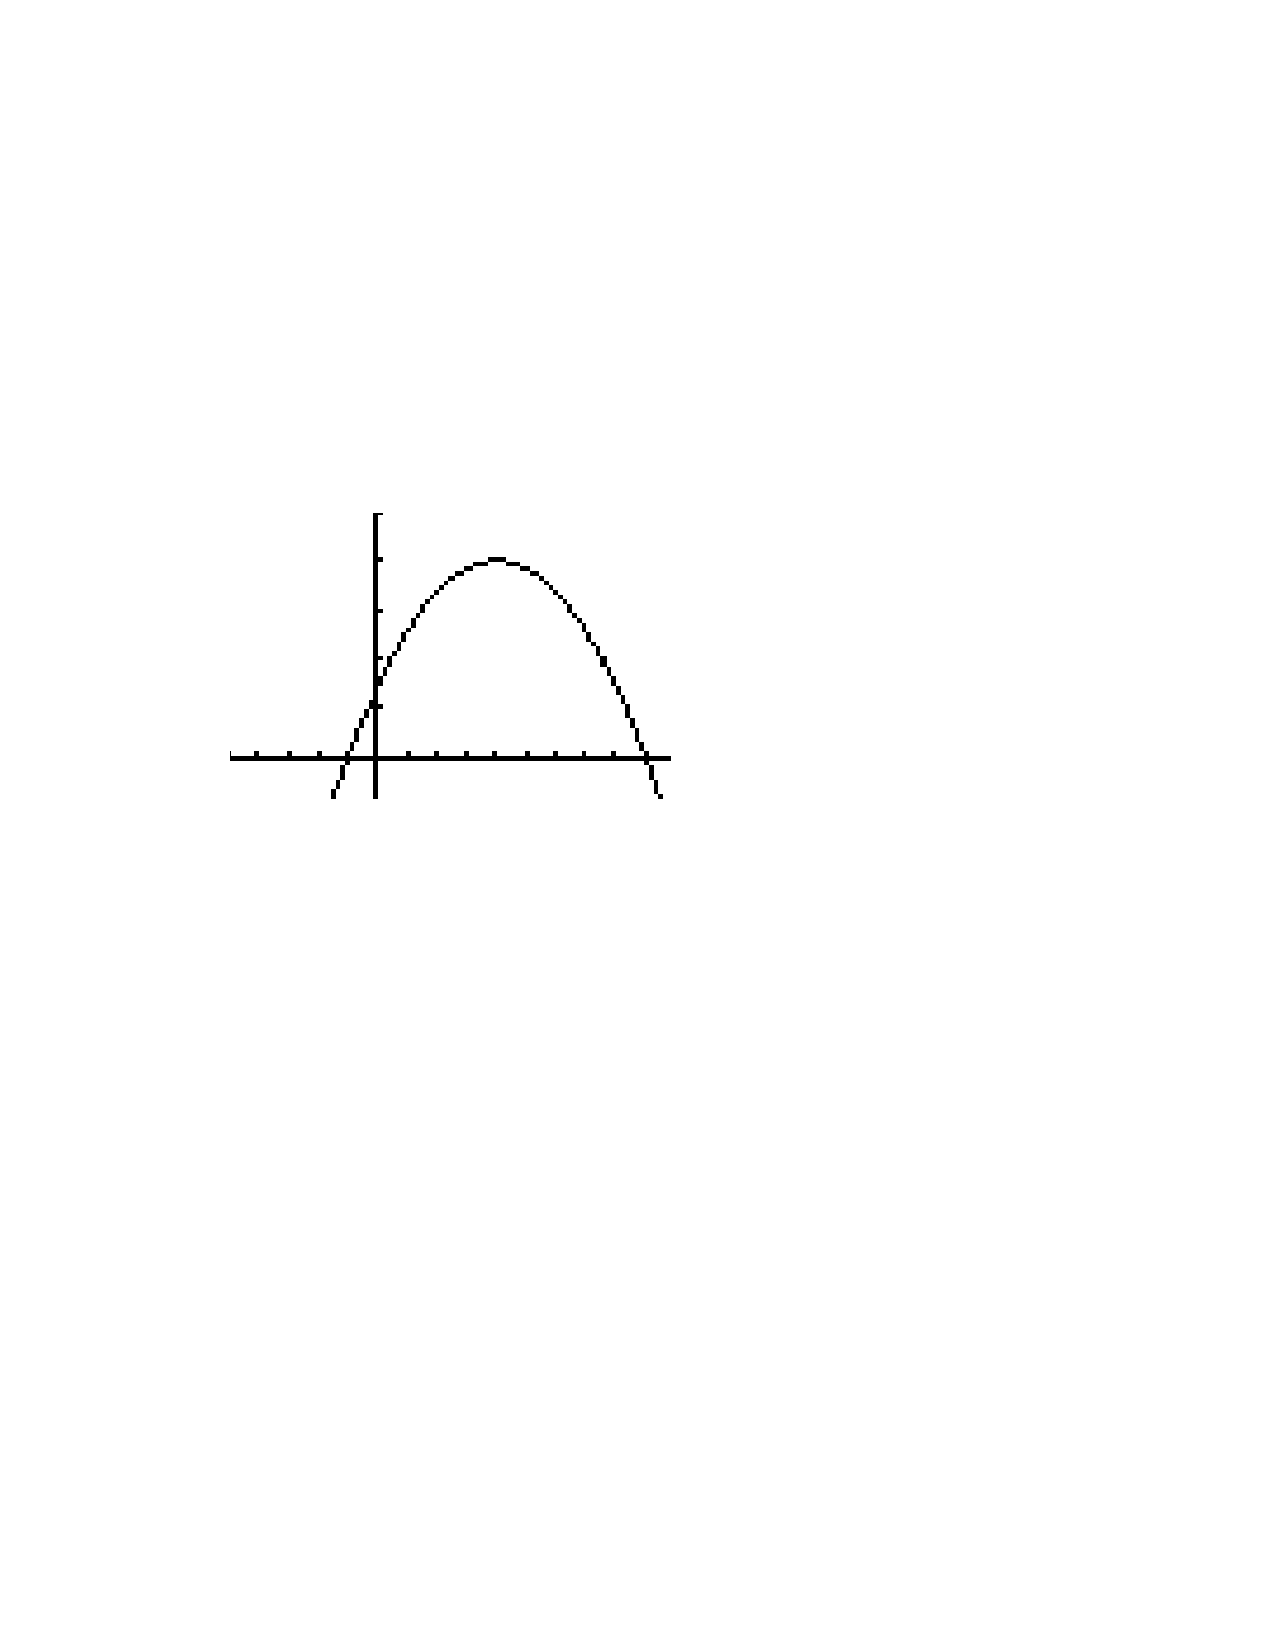
\includegraphics[trim= 170 310 250 180]{Figure1.pdf}
	\end{image}
			\begin{freeResponse}
			Essentially, one just needs to replace all of the $3$'s with $x$'s.  After making this substitution and completing the same algebra, line four becomes
			$$ f'(x) = \lim_{h \to 0} \frac{(x+h)(x-5) - x[(x+h)-5]}{[(x+h)-5](x-5)h}. $$
			
			Multiplying the numerator out and canceling yields
			
			$ f'(x) = \lim_{h \to 0} \frac{-5h}{[(x+h)-5](x-5)h} 
			= \lim_{h \to 0} \frac{-5}{[(x+h)-5](x-5)}
			= \frac{-5}{(x-5)^2}.$
			\end{freeResponse}
\end{problem}
	
	
	
	
			
			

%problem 2			
\begin{problem}
Given the following graph of $f(x)$, find the values where $f(x)$ is zero, positive/negative, increasing/decreasing, and where $f(x)$ has its highest and lowest values.  Additionally, find where the graph of $f(x)$ is the steepest. Then, without sketching the graph of $f'(x)$, determine for which values of $x$ is $f'(x)$ zero, positive/negative, and where $f'(x)$ has the highest and lowest values.  Then sketch $f'(x)$.
	\begin{image}
	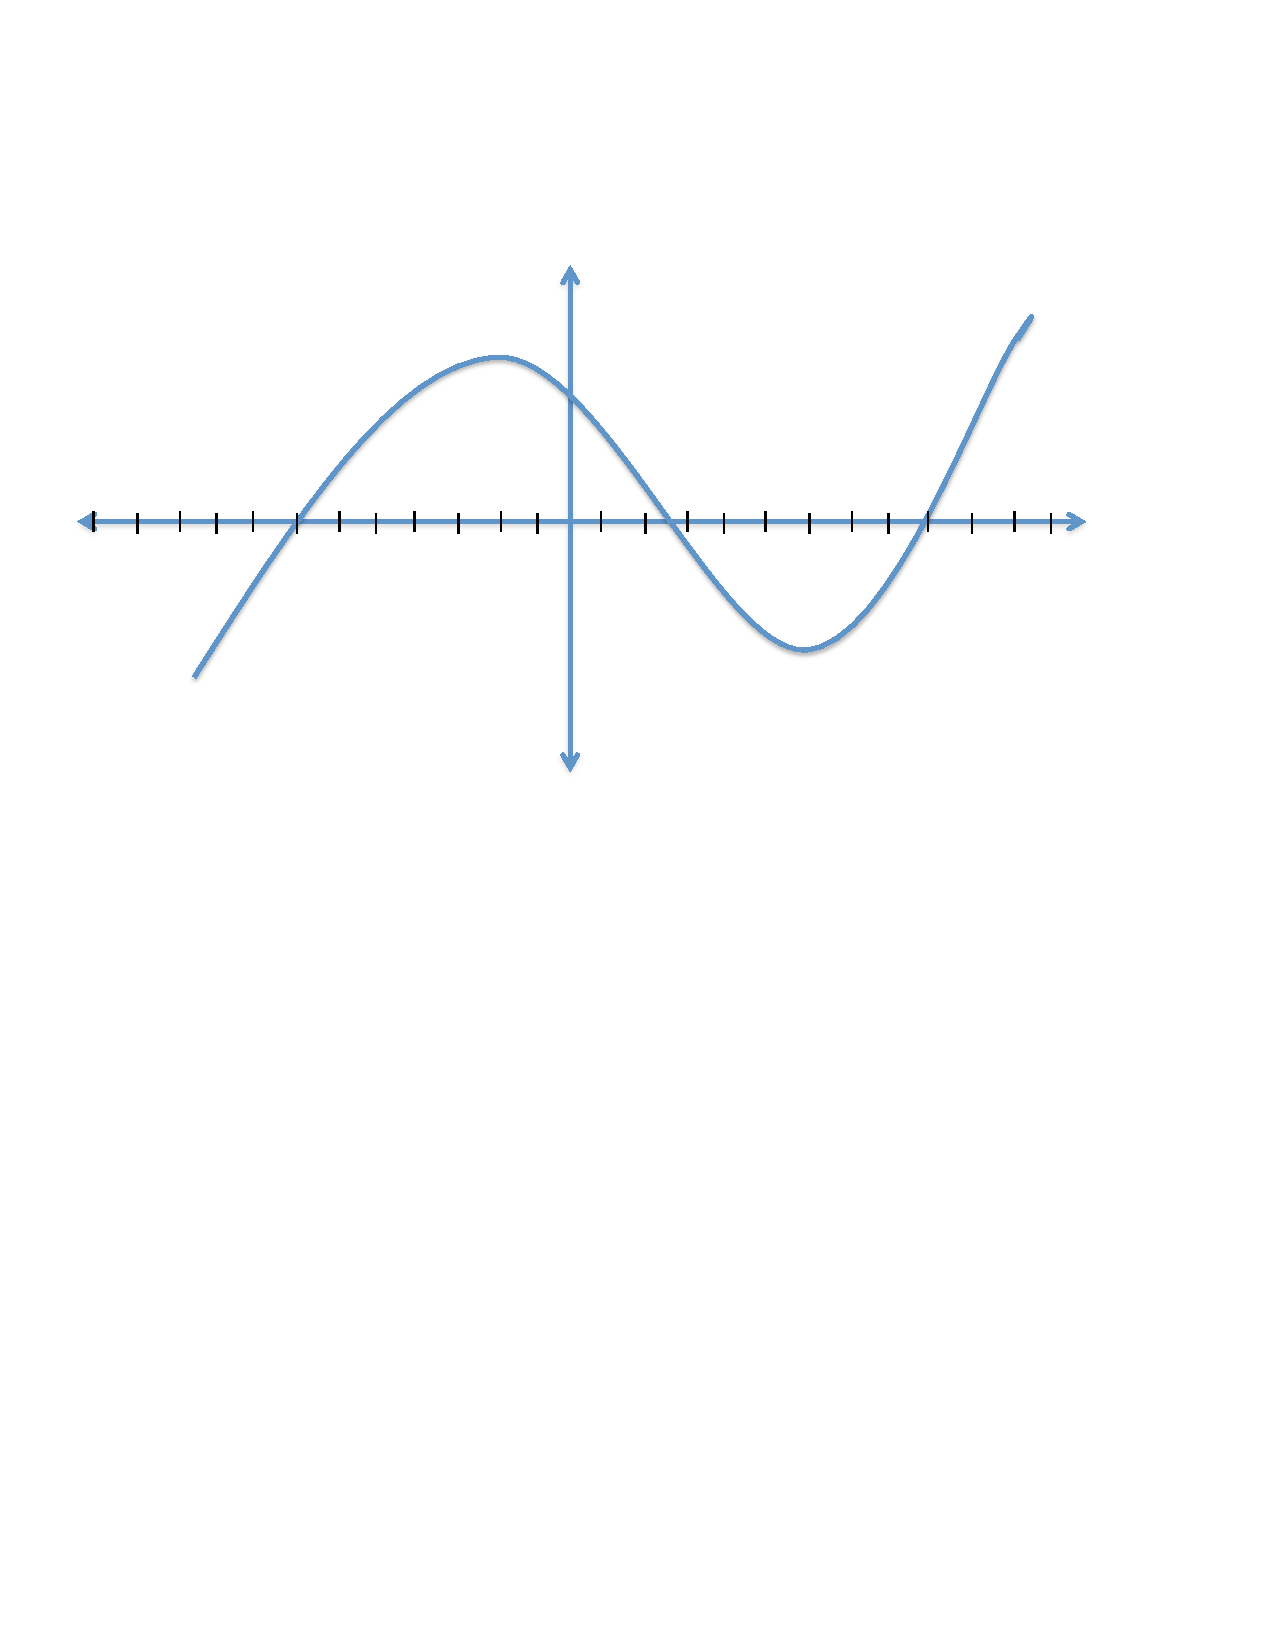
\includegraphics[trim= 170 410 250 100]{Figure2.pdf}
	\end{image}

		\begin{freeResponse}
			\begin{image}
			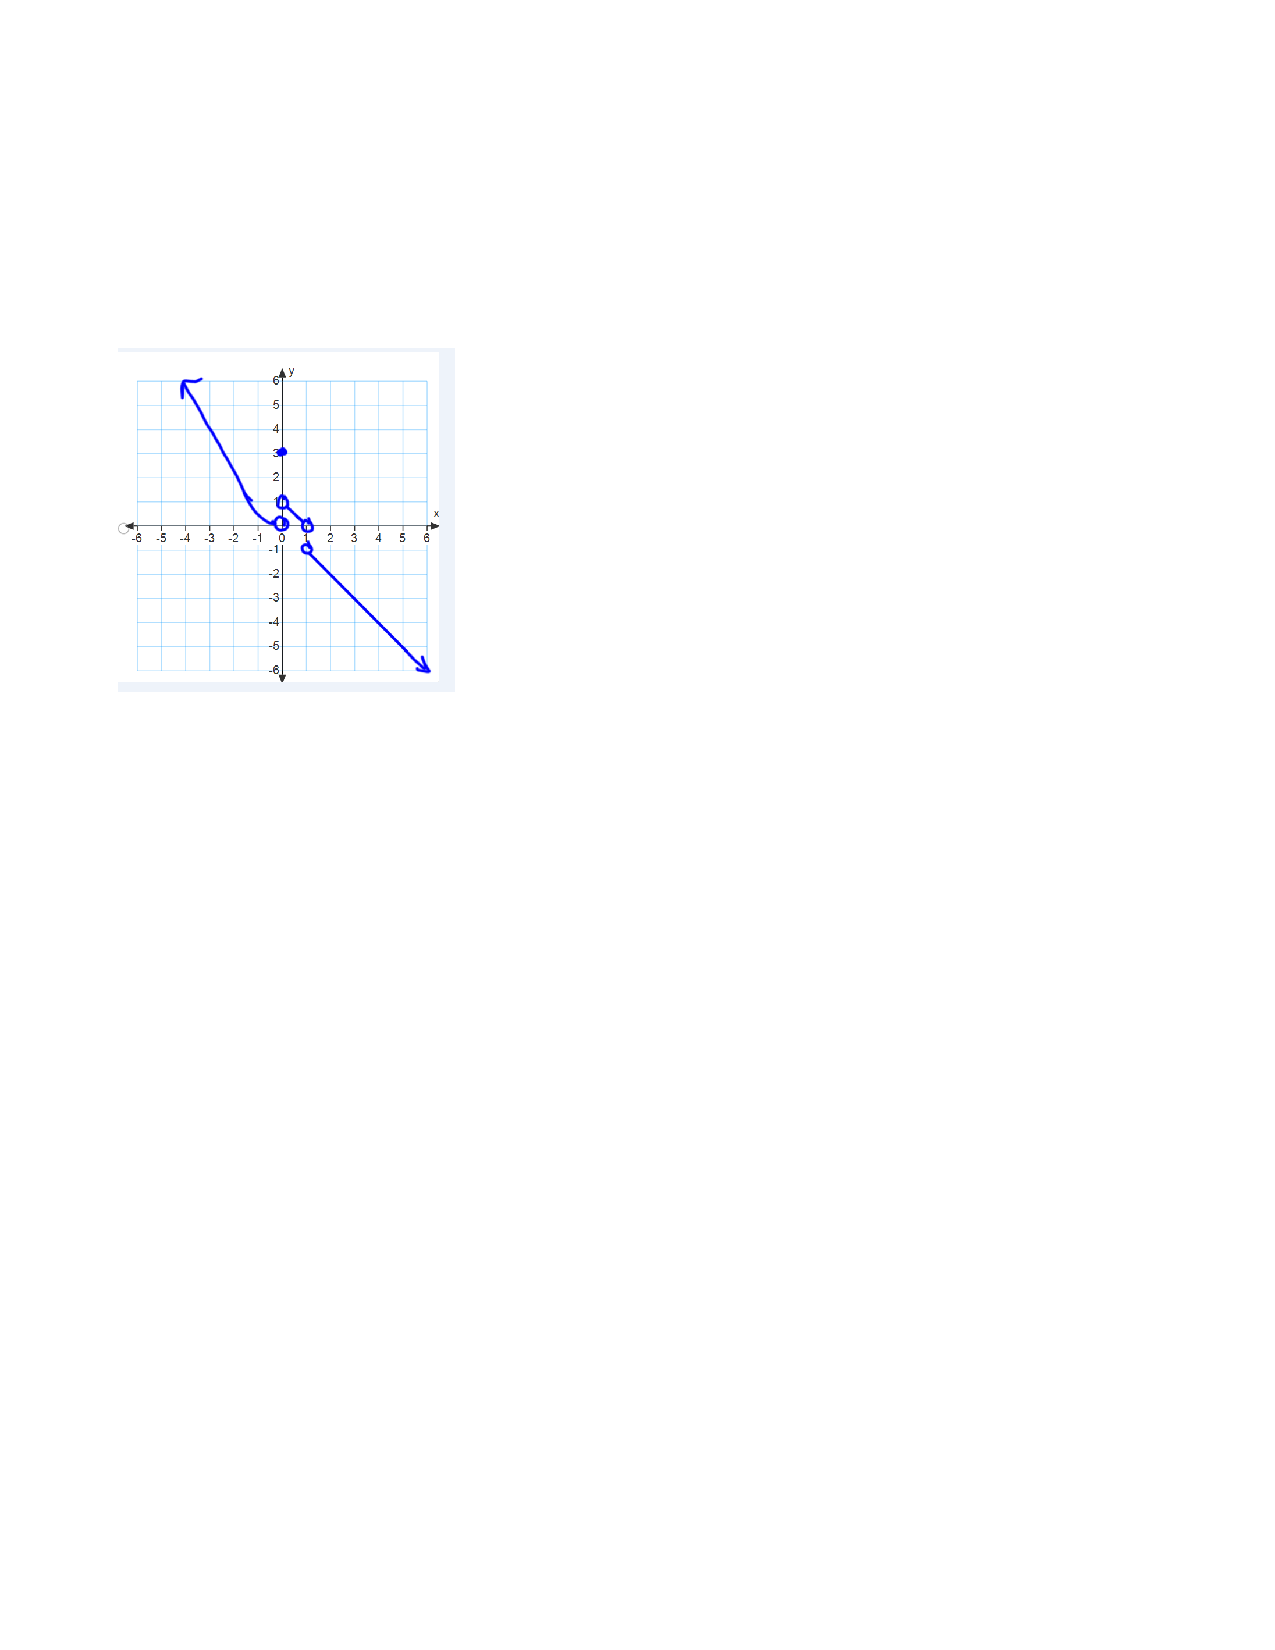
\includegraphics[trim= 250 410 250 160]{Figure3.pdf}
			\end{image}
			
			$f(x)$ is zero when the function crosses the $x$-axis, so at approximately $x=-7,2.75,9$. 
			
			$f(x)$ is negative when the function is below the $x$-axis, so approximately $(-\infty ,-7) \cup (2.75,9)$ .
			
			$f(x)$ is positive when the function is above the $x$-axis, so approximately $(-7,2.75) \cup (9,\infty )$. 
			
			$f(x)$ is increasing on $(-\infty ,-2.5) \cup (6,\infty )$. 
			
			$f(x)$ is decreasing on $(-2.5,6)$.
			
			$f(x)$ (locally) has its highest point at approximately $x=-2.5$.  For $x > 9$, $f(x)$ has no highest point.
			 
			$f(x)$ (locally) has its lowest point at approximately $x=6$.  For $x < -7$, $f(x)$ has no lowest point.
			  
			$f(x)$ is steepest at approximately $x=2$ and $x=8.5$.
			   
			$f'(x)$ is zero when the tangent line has a slope of zero, which is approximately at $x=-2.5$ and $x=6$.  Note, for this question, these are the same answers as the 					(local) highest and lowest point for $f(x)$.   
			   
			${f}'(x)$ is positive when the slope of the tangent line is positive, so when $f(x)$ is increasing which is approximately $(-\infty ,-2.5) \cup (6,\infty )$. 
			   
			${f}'(x)$ is negative when the slope of the tangent line is negative, so when $f(x)$is decreasing which is approximately $(-2.5,6)$.
			   
			${f}'(x)$ has its highest and lowest values when $f(x)$ is steepest, which is approximately when $x=2$ and $x = 8.5$. 
			   
			\begin{image}
			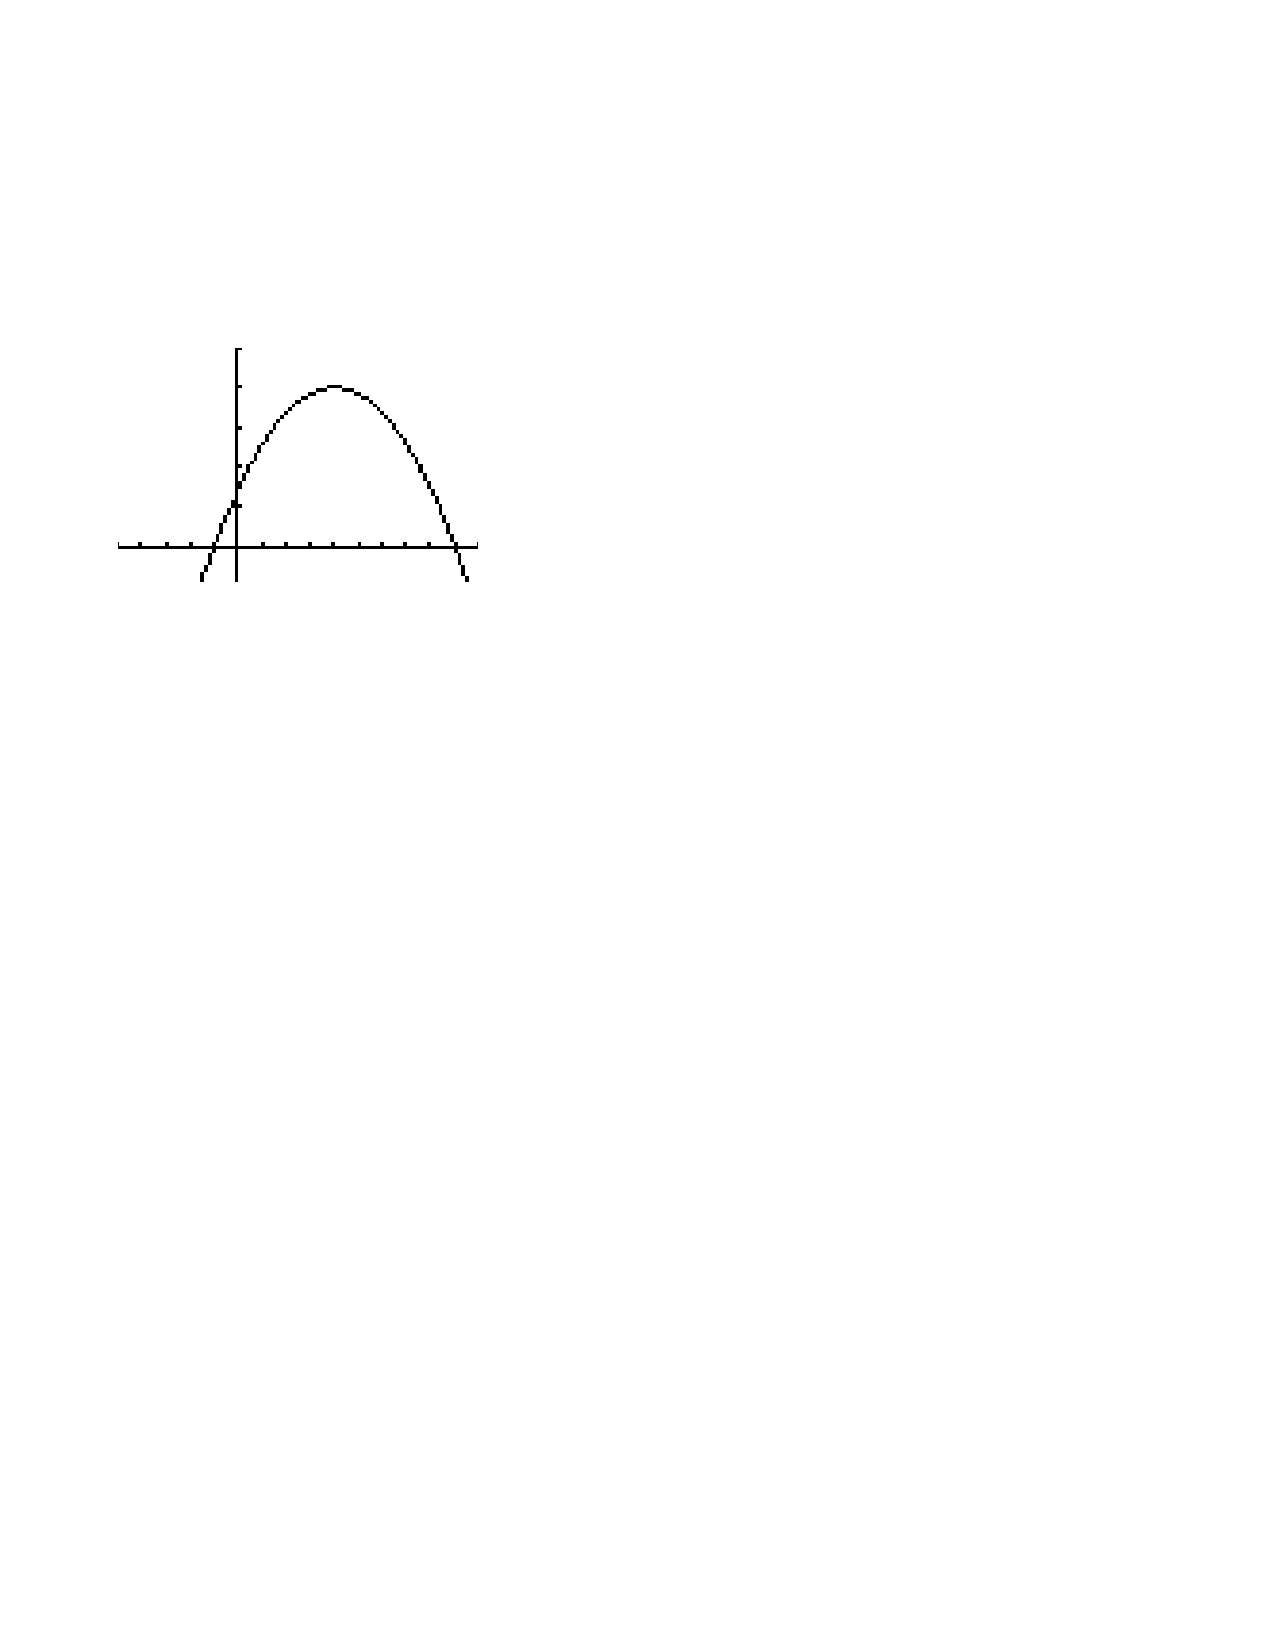
\includegraphics[trim= 170 410 250 190]{Figure4.pdf}
			\end{image}

		
		\end{freeResponse}
		
\end{problem}









%problem 3			
\begin{problem}
Given the graph of $y=f(x)$, sketch the graph of the derivative $f'(x)$.

	\begin{image}
	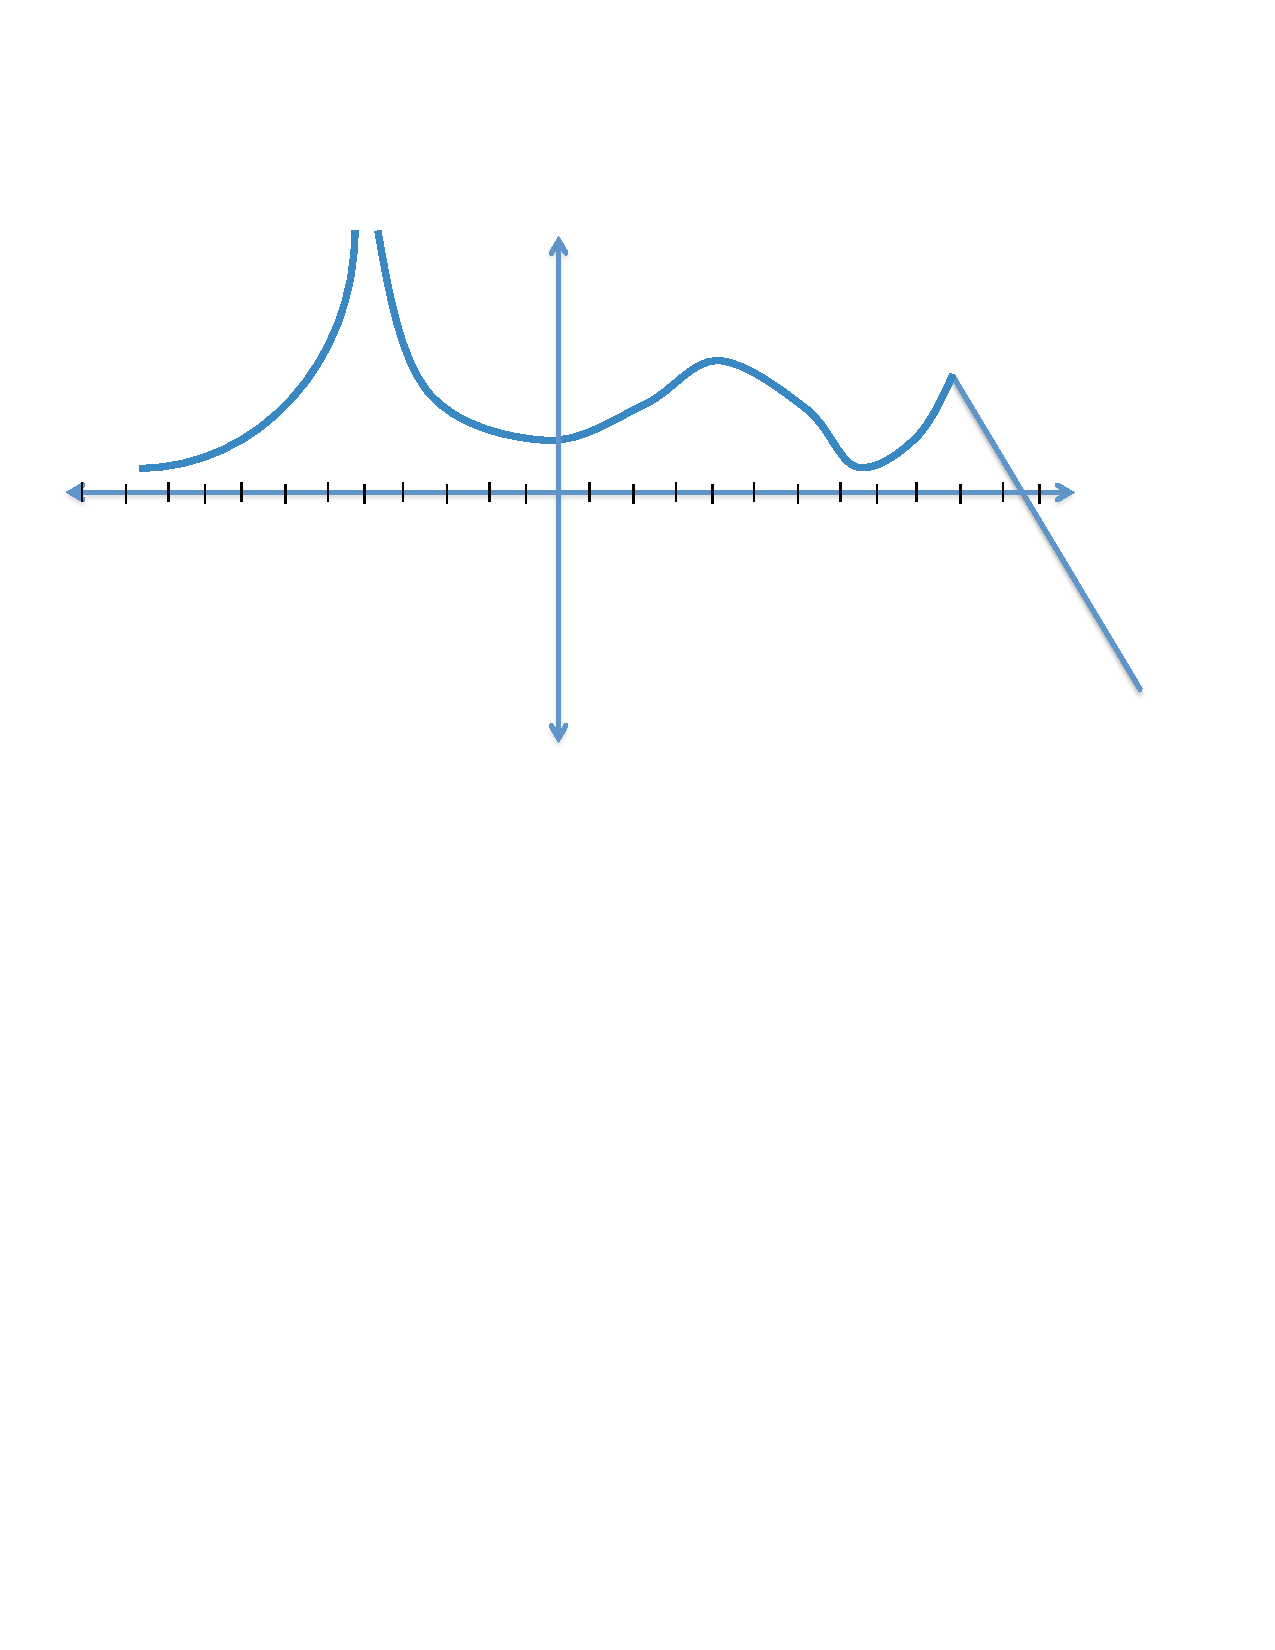
\includegraphics[trim= 220 430 250 110]{Figure5.pdf}
	\end{image}

		\begin{freeResponse}
		The graph of the derivative is in red.  Disclaimer:  despite being drawn on the same graph, the units for $f$ and $f'$ are \dfn{not} the same!
		
			\begin{image}
			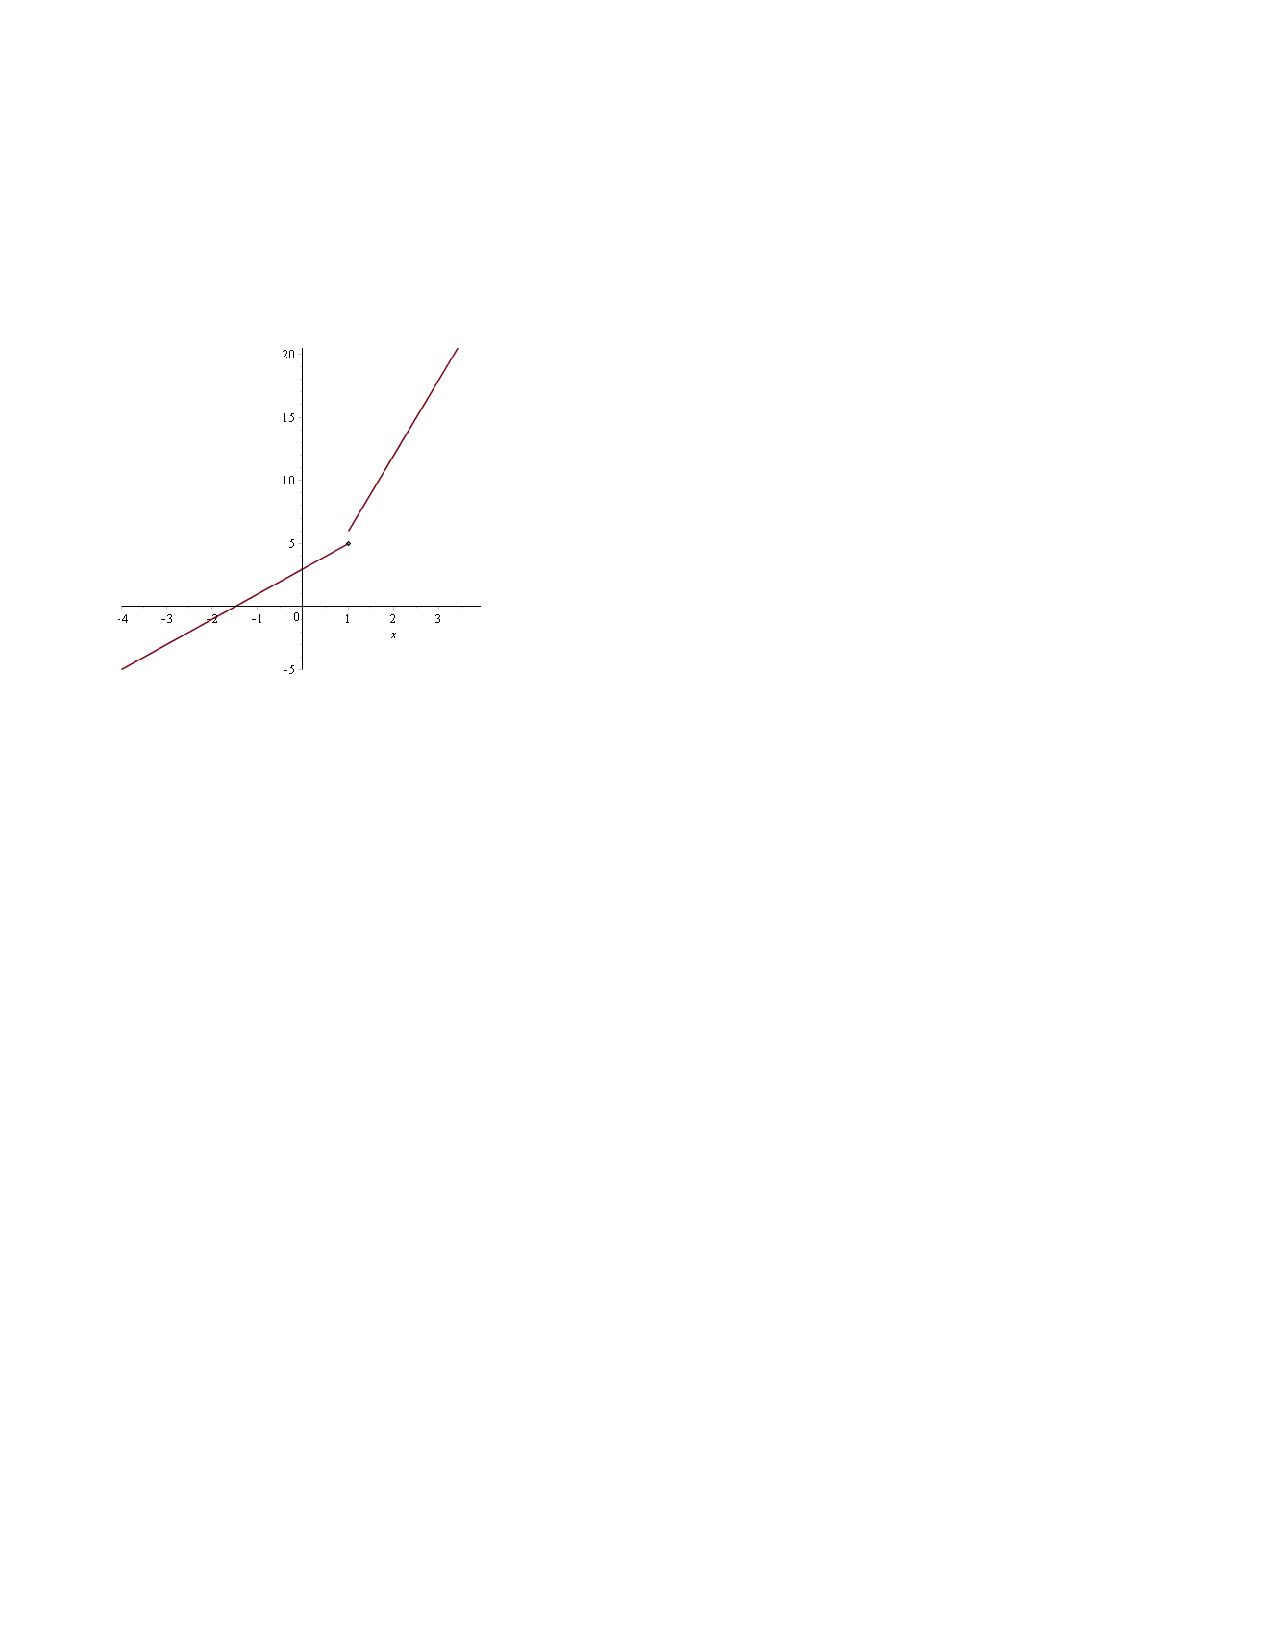
\includegraphics[trim= 220 410 250 195]{Figure6.pdf}
			\end{image}
			
		\end{freeResponse}
		
\end{problem}







%problem 4
\begin{problem}
Use the graph of $g$ in the figure to do the following.
	\begin{enumerate}
	
	\item Find the values of $x$ in $(0,4)$ at which $g$ is not continuous.
		\begin{freeResponse}
		$g$ is not continuous at $x=1$.
		\end{freeResponse}
		
		
	
	\item Find the values of $x$ in $(0,4)$ at which $g$ is not differentiable.
		\begin{freeResponse}
		$g$ is not differentiable at $x=1$ and $x=2$.
		\end{freeResponse}
		
		
	
\begin{tikzpicture}

%\draw[help lines] (-1,-1) grid (5,5);

\draw [->] (-1,0) -- (5,0);
\draw [->] (0,-1) -- (0,5);

\draw (1,0.1) -- (1,-0.1);
\draw (2,0.1) -- (2,-0.1);
\draw (3,0.1) -- (3,-0.1);
\draw (4,0.1) -- (4,-0.1);
\draw (-0.1,1) -- (0.1,1);
\draw (-0.1,2) -- (0.1,2);
\draw (-0.1,3) -- (0.1,3);
\draw (-0.1,4) -- (0.1,4);

\draw (1,-0.1)node[below]{$1$};
\draw (2,-0.1)node[below]{$2$};
\draw (3,-0.1)node[below]{$3$};
\draw (4,-0.1)node[below]{$4$};
\draw (5,0)node[below]{$x$};
\draw (-0.1,1)node[left]{$1$};
\draw (-0.1,2)node[left]{$2$};
\draw (-0.1,3)node[left]{$3$};
\draw (-0.1,4)node[left]{$4$};
\draw (-0.1,5)node[left]{$y$};

\draw (3,3.5)node{$y = g(x)$};

\draw[red, very thick] (2,2) arc [radius=1, start angle=0, end angle = 180];
\draw[red, very thick] (4,2) arc [radius=1, start angle=0, end angle = 180];

\draw[fill=white] (1,3) circle [radius=0.075];


\end{tikzpicture}
	
	\end{enumerate}



\end{problem}
	
	
	
	
	
	
	
	
	

	










								
				
				
	














\end{document} 


















